\chapter{The~\texttt{porthos2}:~implementation}
\label{ch:impl}

The main reason for commencing the work on \porthos[2] was the need for processing real-world C programs, which, at first, requires the input language to be extended.
This implies the support not only for new syntactic structures of C language (such as the \texttt{switch} statement or the postfix increment operator \texttt{i++}), but also for its fundamental concepts and features (such as types, pointer arithmetic or first-order functions), which requires revision of the whole architecture of the tool.
Although far not the entire C language has been supported (that, considering its complexity and numerous pitfalls, goes far beyond current thesis%
\footnote{To ensure that, we have merely to look at existing C compilers, for instance, the open-source \texttt{gcc} compiler, that uses a C parser written in more than 18.5 thousand lines (see \url{https://github.com/gcc-mirror/gcc/blob/master/gcc/c/c-parser.c})}%
), we consider the accomplished work as a step towards this.
%This applies not only to instances that simply constitute the syntactic sugar of C language (such as the \texttt{switch} statement or the prefix increment operator \texttt{++i}), but also to its fundamental concepts and features (such as pointer arithmetic or structures).
%However, the architecture of current version of \porthos{} does not allow to ... as it is ....
% Although and optimisation of the tool so that it is able to process real C programs in perspective.

%In current Chapter we discuss the new architecture of \porthos[2].

% function invocations/calls: inlining with binding
% contexts: for now, no ctxs
% comparing to cprover (https://www.cprover.org/cbmc/doc/manual.pdf, page 45, absatz about 'goto') where "the loop is unwound a given number of times" , we SHOULD have 2 modes of unrolling: 1) number of times, and 2) number of high-level instructions executed
% TODO(code): (https://www.cprover.org/cbmc/doc/manual.pdf, page 45) "The break and continue statements are replaced by equivalent goto statements as described in the ANSI-C standard."

% TODO: arrays: cprover manual page 48


%\section{The architecture of \porthos[1]}
\section{General principles}
\label{ch:impl:principles}

The existing implementation of \porthos[1] does not distinguish the event-based program model from the high-level AST, they both are encoded into single SMT-formula (see classes of package `\texttt{dartagnan.program}' of \porthos tool).
Moreover, the syntax tree was implemented as a mutable data structure, which is being modified at all stages of the program (for instance, see the methods `\texttt{dartagnan.program.Program.compile(...)}' of \porthos{} that recursively compute some properties of the AST and change its state).
We are inclined to consider this architecture as one that is fast to develop, but hard to maintain (since it is difficult to guarantee the correctness of the program) and extend (since adding the support for a new high-level instruction requires changing multiple components of the program, from parser to encoder).
%Moreover, we encounter serious problems when we need to add support for control-flow jumps (as \texttt{continue}, \texttt{break}, \texttt{goto} in C).

% todo: in old porthos the strategy soft: print info about error. new: exception on any detected violation of any invariant

Therefore, while working on the new design of \porthos[2], we decided to clearly separate the high-level intermediate code representation (implemented as a recursive AST structure) from low-level event-based representation (implemented as an event-flow graph).
Such a modular architecture allows to support multiple input languages by parsing them and converting parsed syntax trees to a simplified AST. which, along with all other data-transfer objects (DTO), must be immutable, so that it is possible to guarantee the correctness of the program by controlling its invariants.
The immutability in \porthos[2] is implemented via \texttt{final} fields that are assigned by the immutable-object values (either a primitive type, or another immutable object, or an immutable collection provided by the library Guava by Google%
\footnote{Guava project repository: \url{https://github.com/google/guava/}}%
).

During the development of \porthos[2] we mainly followed the \textit{KISS~principle}, which can be exhaustively described in 17 Unix Rules of Eric Raymond~\cite{raymond2003art}.% which include the rule of modularity, the rule of clarity, transparency, extensibility, etc.
The following list summarises the main rules we followed during the development of \porthos[2]:

\vspace{0.5em}
\begin{enumerate}[nolistsep]
  \item \textit{Robustness:}
    \begin{enumerate}[label*=\arabic*.]
      \item usage of immutable data structures for all DTOs;
      \item interrupting the work on errors;
      \item modular architecture: each module can be tested independently;
      \item usage of software design patterns if necessary;
    \end{enumerate}
  \item \textit{Transparency:}
    \begin{enumerate}[label*=\arabic*.]
      \item following the principles of simplicity and readability;
      \item clear and informative program output;
    \end{enumerate}
  \item \textit{Efficiency:}
    \begin{enumerate}[label*=\arabic*.]%[leftmargin=1.5em]
      \item keeping the trade-off between execution time and memory usage;
    \end{enumerate}
  \item \textit{Extensibility:}
    \begin{enumerate}[label*=\arabic*.]%[leftmargin=1em]
      \item clear modular architecture.
    \end{enumerate}
\end{enumerate}


As \porthos[1], the \porthos[2] uses the open-source SMT solver \texttt{Z3} from Microsoft Research~\cite{de2008z3}. However, unlikely its predecessor, the \porthos[2] has an additional abstraction level \zformula{} (see Section~\ref{ch:impl:model:zformula}) that allow to use any other SMT solver. %TODO: *should* allow?

The programming language choice for \porthos[2] was also made in favour of \textit{java}, firstly, in order to be able to reuse some parts and concepts of \porthos[1] that is written in java, and secondly, because the authors find the object-oriented (OOP) concepts of java suitable for modelling languages.
Although java does not show best results in performance benchmarks (for example, comparing to C++~\cite{hundt2011loop, oaks2014java}), the performance cornerstone of \porthos[2] (as well as any other SMT-based code analyser) is the phase of solving the SMT-formula, which is left to the third-party SMT-solver \textit{Z3}%
\footnote{The Z3 project repository: \url{https://github.com/Z3Prover/z3}} %
invoked from \porthos[2] via java API.
However, considering the perspective of using \porthos[2] as a static analyser for real-world programs, the memory optimisation problem must also be taken into account during both encoding and solving stages.
It is worth noting that, for the reasons of simplicity, the \porthos[2] is not a concurrent program, however, we believe that, due to its modular architecture, it can be easily parallelised on the level of program modules.


\section{General architecture}
\label{ch:impl:arch}

The general architecture scheme of \porthos[2] is presented in Figure~\ref{fig:arch}.
The program takes as input the program to be analysed and one (the reachability analysis mode) or two (the portability analysis mode) memory models. The parsed program syntax tree is then converted (Section~\ref{ch:impl:proc:y-constr}) to a program AST called \ytree{}%
\footnote{In order to avoid confusion between different internal representations, we prefix the names of elements of each internal representation with a letter. For instance, we picked the letter `Y' to denote the AST code representation as drawing of this letter resembles the tree branching; with letter `X' we prefix elements of the event-flow graph as the events are to be e\textbf{x}ecuted; and with letter `W' we prefix elements of the \textbf{w}eak memory model AST.} %
(Section~\ref{ch:impl:model:ytree})
%, and the memory model is being parsed (Section~\ref{ch:impl:proc:w-parser}) to another AST called \wmodel{} (Section~\ref{ch:impl:model:wmodel}).
, which then is being pre-processed at the pre-compilation stage (Section~\ref{ch:impl:proc:x-pre-compiler}) in order to collect information necessary for the compilation.
The \ytree{} then is being compiled (Section~\ref{ch:impl:proc:x-compiler}) to an \xgraph{} representation (Section~\ref{ch:impl:model:xgraph}).
The compiled \xgraph{} then undergoes a number of transformations (Section~\ref{ch:impl:proc:x-transf}) necessary for the encoding into a \zformula{} (Section~\ref{ch:impl:model:zformula}) at the pre-encoding stage (Section~\ref{ch:impl:proc:x-transf}).
Then, the memory-model constructor (Section~\ref{ch:impl:proc:w-constr}) constructs the derived relations on the basis of the \xgraph{} in order to build the weak memory model \wmodel{} (Section~\ref{ch:impl:model:wmodel}).
Thereafter, \wmodel{} and transformed \xgraph{} are encoded (Section~\ref{ch:impl:proc:z-encoder}) to a \zformula{} representation (a wrapper over an SMT logical formula), which then is passed as an input to the SMT-solver.

\begin{figure}[H]
  \centering
  % TODO: remove scale 0.8 if it can fit the whole page
  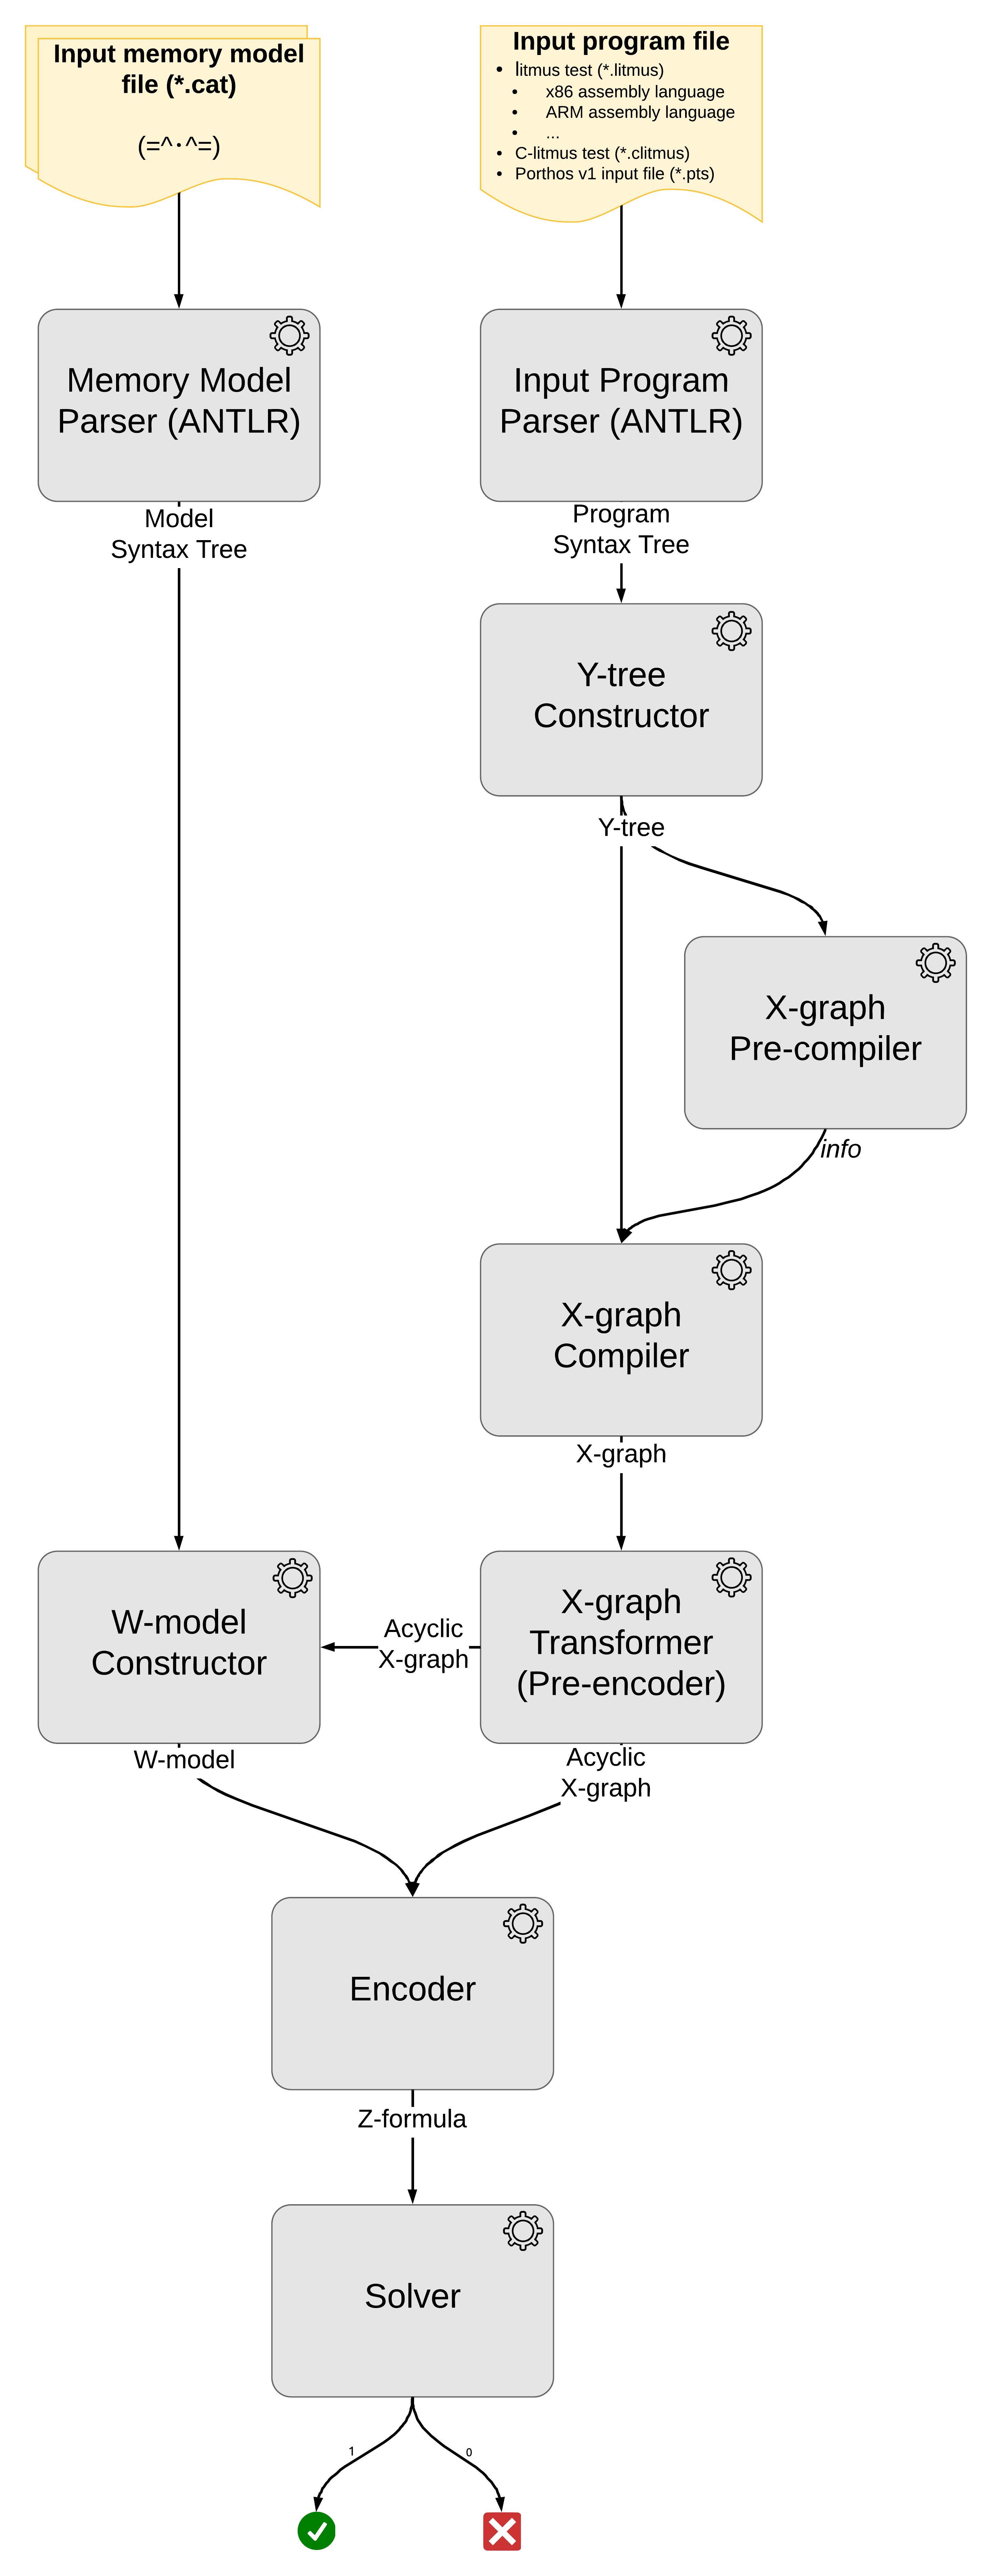
\includegraphics[width=\textwidth,height=0.8\textheight,keepaspectratio]{img/my/lucidchart.com/data-flow-vert-300dpi.png}
  \caption{General architecture of \porthos[2]}
  \label{fig:arch}
\end{figure}


\subsection{The program input}
\label{ch:impl:input}
%(for instance, the original input language of \porthos{} tool, two variants of syntax of a litmus test used by \tool{herd}, an assembly language for any supported architecture).

Both \porthos[1] and \porthos[2] use the ANTLR parser generator%
\footnote{The ANTLR project repository: \url{https://github.com/antlr/antlr4}}%
~\cite{parr2013definitive}, a~powerful language processing tool.
The ANTLR takes as input the user-defined grammar of the target language in a BNF-like form and produces the LL(*)-parser and optionally some auxiliary classes (such as listeners and visitors for the syntax tree).
Although this parser may be not as efficient as the hand-written language-optimised parser, it reduces the overhead of implementing the parser significantly.
Among other advantages ANTLR, it is worth of noting that it has rather large collection of officially supported grammars. Nonetheless, the intuitive syntax for defining grammars and numerous of tools for debugging grammars make the ANTLR an attractive instrument for solving the parsing problem.

Figure~\ref{fig:in_grammar_pts} represents the simplified grammar of of input language used by previous version of \porthos{} (the full ANTLR grammar is available at Appendix~\ref{apx:grammar}.

\begin{figure}[h]%[!hb]
\centering
\begin{lstlisting}[mathescape=true,%
                  caption={The sketch of the input language grammar used by \oldporthos},%
                  label={fig:in_grammar_pts},%
                  morekeywords={if,then,else,return,while,program,thread},%
                  breaklines=true,%
                  basicstyle=\ttfamily\scriptsize]
<prog> : <init> <thrd>* <assert>
       ;
<thrd> : thread <tid> <inst>
       ;
<inst> : <atom>
       | <inst> ; <inst>
       | while <pred> <inst>
       | if <pred> { <inst> } <inst>
       ;
<atom> : <reg> <- <expr>
       | <reg> <:- <loc>
       | <loc> := <reg>
       | <reg> = <loc>.load(<atomic>)
       | <loc> = <reg>.store(<atomic>)
       | 'mfence'
       | 'sync'
       | 'lwsync'
       | 'isync'
       ;
<pred> :
       | true
       | false
       | <expr> (and | or) <expr>
       | <expr> ('==' | '!=' | '>' | '>=' | '<' | '>=') <expr>
       ;
<expr> : [0-9]
       | <reg>
       | <expr> ('*' | '+' | '-' | '/' | '%') <expr>
       ;
\end{lstlisting}
\end{figure}

The input language parser used by \porthos[1] suffered from several disadvantages.
Firstly, it contained the parser code inlined into directly the grammar, so that the grammar would serve as a template for the parser code (which is called semantic actions). Such a combining of two rich languages%
\footnote{by the term "reach" we mean "expressiveness": at least, the grammar of the language of semantic actions (i.e., java in our case) is Turing-complete.} %
makes the code hardly understandable, and, therefore, poorly maintainable. In \porthos[2], we clearly separated the parser (generated from the grammar file `\textit{<grammar>.g4}') from the converting the ANTLR syntax tree to the AST, that is one for all  languages of an input program.

Secondly, the semantics of operations was defined syntactically, whereas processing programs written in most modern languages (including C) requires the semantics resolution based on typification%
\footnote{for instance, given two functions
`\lstinline{int foo(int a)}' and `\lstinline{int foo(char a)}', the code `\lstinline{int a = '1'; foo(a);}' will invoke the first method rather than the second one.}.%
As the reader can notice from the grammar sketch in Figure~\ref{fig:in_grammar_pts}, the memory operations of different kinds vary syntactically. For example, the assignment of local computation to a register uses the symbol `\lstinline{<-}', the atomic non-relaxed load operation denoted as `\lstinline{<:-}', non-relaxed store operation denoted as `\lstinline{:=}', and the semantics of relaxed \lstinline{load} and \lstinline{store} are resolved syntactically by matching the method name. In \porthos[2], the semantics of the data-flow operation is determined according to the types of operands, that are determined during the pre-compilation stage (see Section~\ref{ch:impl:proc:x-pre-compiler}). The semantics of the methods also is being resolved during the pre-compilation stage via the \textit{invocation hooks} mechanism (see Section~\ref{ch:impl:proc:x-pre-compiler:hooks}).

Thirdly, the grammar used by \porthos{} had restricted set of allowed operations. For example, it allowed only computations over the local variables, which might lead to inconsistency of the result SMT-formula if the same variable name was used both as a register and as a location, for instance, the in code snippet `\lstinline{x := reg1; reg2 <- (x + 1);}', the first statement interprets the variable \lstinline{x} as a location, while the grammar of second statement requires it to be a register. Also, only integers were processed by the input language parser of \porthos[1]. In \porthos[2], we extended support for primitive types supported by the \texttt{Z3} solver (this apply to 32-bit integers encoded as \texttt{Int}s, floats encoded as \texttt{Real}s, enums encoded as Z3 \texttt{Scalars}).
%TODO : constant arrays? https://rise4fun.com/Z3/tutorial/guide
Thus, adding support for more advanced syntactic structures as pointers, arrays, function definitions and calls was one of the purposes of revising the tool architecture.

The minor drawbacks of grammar used by \porthos[1] include lack of operator associativity (expressions of type \lstinline{1 + 2 * 3} could not be parsed), incorrectly (in terms of C) implemented grammar rule for statements (the semicolon punctuator `\lstinline{;}' was implemented as the separator between two statements, whereas in C it serves as a statement terminator). Also, \porthos[1] supports only the litmus-specific syntax for the variables initialisation, however, it allows only ini
tialisation of the shared variable and only by default value \lstinline{0}. The \porthos[2] supports arbitrary declaration to be performed in initialisation statement.


The \porthos[2] uses the C language grammar of proposed in the C11 standard~\cite{jtc2011sc22}, that was extended by litmus test-specific syntax such as initialisation and final-state assertion statements (the original ANTLR grammar can be found in the official repository containing the collection of ANTLR v4 grammars~\footnote{Repository path: \url{https://github.com/antlr/grammars-v4}}).
Currently, \porthos[2] can operate only in the intra-procedural analysis mode (analysing single procedure), assuming that each function defined in the input file is being executed in a separate thread.
However, the redesigned architecture of \porthos[2] allow to easily support inter-procedural (cross-procedure) analysis by inlining function calls and binding variable contexts. Also, Current version of \porthos[2] simply ignores C processor directives, however, in future it is possible to support it.

%TODO: say sth about 100500 litmus-tests for kernel


\subsection{The internal representations}
\label{ch:impl:model}
%As it has already been mentioned, all internal representations constructed by \porthos[2] are \textit{immutable}.

\subsubsection{Y-tree}
\label{ch:impl:model:ytree}

- TODO: everything inherited YEntity + citation

The first internal representation that \porthos[2] uses is the \ytree{}, which represents a rather high-level AST.
The Apendix~\ref{apx:trees} represents the file tree of main classes that constitute the \ytree{} hierarchy (as the inheritance tree might be obvious for the C-like AST, we confine ourselves to representing the classes file tree only).

%\columnratio{0.7}%\begin{paracol}{2}
%\switchcolumn%\VerbatimInput{inc/lst/Ytree-tree.out}%\end{paracol}
The abstract syntax tree \ytree{} is an abstraction level suitable for compiling to a low-level representation (in case of processing low-level assembly code, it may be directly converted to the \xgraph{} representation).
As the ANTLR syntax tree follows the same structure as the grammar, which is a superset of the real (meaningful) grammar of C language, it lacks multiple concepts of the language (for example, the syntax of indexer access corresponds the grammar rule \lstinline{postfixExpression '[' expression ']'}, that is converted to the \texttt{YIndexerExpression}).
However some details of the syntax might have been abstracted away (for instance, array operations may be emulated by functions invocations, see~\cite{gries2012science}\textbf{TODO:CHAPTER,PAGE}), we found this level of abstraction as suitable enough for our tasks.

Following the terms of C standard, we distinguish \textit{statements} (actions to be performed) and \textit{expressions} (TODO).

- TODO: all statements inherit \texttt{YStatement} + interface lstlisting

The \porthos[2] processes the following statements: 
\begin{itemize}[nolistsep]
  \item \texttt{YBranchingStatement} representing the \texttt{if-then-else} statement,
  \item \texttt{YLoopStatement} representing both \texttt{while}- and \texttt{for}-loops, %TODO:RENAME YWhileLoopStatement->YLoopStatement in code!!!)}
  \item \texttt{YJumpStatement} representing unconditional jump (\texttt{goto}-jump to a label and loop-jumps \texttt{break} and \texttt{continue}),
  \item \texttt{YCompoundStatement} (block statement) representing sequence of \texttt{N} statements grouped into one syntactic unit,
  \item \texttt{YLinearStatement} representing single expression.
\end{itemize}

According to the C standard, \textit{"any statement may be preceded by a prefix that declares an identifier as a label name"}.
However, the \ytree{} statements may have only simple symbolic labels, which have to be resolved at the pre-compilation stage.
Apart from the listed set of statements, \ytree{} has also the \texttt{YFunctionDefinition} and its litmus-specific inheritor \texttt{YProcessStatement} used in intra-procedural analysis mode.
The function definition contains the \texttt{YCompoundStatement}-typed body and the signature of type \texttt{YMethodSignature}, which is used in the function resolution during the compilation stage. %TODO: pre-compilation?
The other litmus-specific statements are \texttt{YPreludeStatement} that carries the list of \texttt{YStatement}-typed initial writes, and \texttt{YPostludeStatement} that carries the \texttt{YExpression}-typed binary expression to be asserted by the litmus test.

Similar to statements of \ytree{}, its expressions 

pointer operations are modeled as the pointer level of and expression (although it is the property of type, the y-tree is untyped, so elements that represent syntactic expressions shoudl carry tnis information)



Each element of \ytree{} carries the \texttt{OriginLocation} %
\textbf{(TODO: Rename CodeLocation->OriginLocation in the code!)} %
instance that contains information about the coordinates of the input text that generated the \ytree{} element.


\subsubsection{X-graph}
\label{ch:impl:model:xgraph}

\subsubsection{W-model}
\label{ch:impl:model:wmodel}

\subsubsection{Z-formula}
\label{ch:impl:model:zformula}


\subsection{The processing units} %Transformation}
\label{ch:impl:proc}

\subsubsection{Input program parser}
\label{ch:impl:proc:inp-prog-parser}
% todo: test pre-/post-fix operations //+think how current tool will behave if there's more than one post-operation //and pre-operation


\subsubsection{Input memory model parser}
\label{ch:impl:proc:inp-mod-parser}

\subsubsection{Y-tree constructor}
\label{ch:impl:proc:y-constr}

The ANTLR syntax tree of C

%, comparing to ANTLR syntax tree, does not have 
- desugar, equiv transform
- variables distinguished from 


\subsubsection{X-graph pre-compiler}
\label{ch:impl:proc:x-pre-compiler}

\paragraph{Invocation hooks}
\label{ch:impl:proc:x-pre-compiler:hooks}

\subsubsection{X-graph compiler}
\label{ch:impl:proc:x-compiler}

\subsubsection{X-graph transformer}
\label{ch:impl:proc:x-transf}

\subsubsection{W-model constructor}
\label{ch:impl:proc:w-constr}

\subsubsection{Z-formula encoder}
\label{ch:impl:proc:z-encoder}

%todo: mention The SMT-LIB standard http://smtlib.cs.uiowa.edu/papers/smt-lib-reference-v2.6-r2017-07-18.pdf


\subsection{The program output}
\label{ch:impl:out}


%TODO: say sth about syntax errors handling: still now, what if parser does not accept syntax?

- if we don't support , our parser still parses it, and the error is thrown at the moment of converting syntax tree to the AST (Y-tree).

- So, The language-dependent syntax tree is converted to the AST by the stateless Visitor (e.g., for C11->Ytree conversion is made by 'C2YtreeConverterVisitor') + short structure of this visitor (how?.. need ly?)


%\section{The Y-tree: an AST}
%\label{ch:impl:ytree}

- picture of the Y-hierarchy. everything inherits interface YEntity

- immutable

- AST is untyped (YVariableRef).

- short characteristics with citations from the code (this AST contains very basic language elements according to the C execution model (statements and expressions) )

- minor changes are performed by converting to ytree representation: desugaring the target code, etc. (what else?)


%\section{Model parser}
%\label{ch:impl:model}

TODO


\section{Compiling the Y-tree to the X-graph}
\label{ch:impl:y2x}


\begin{figure}%[!b]%[H]
  \centering
  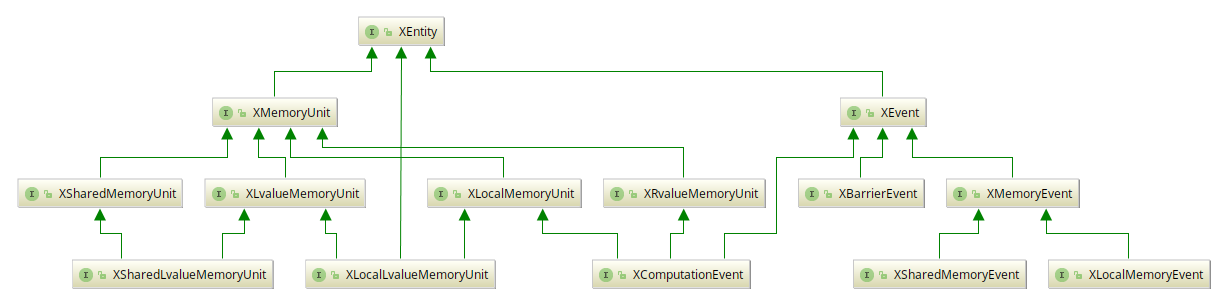
\includegraphics[width=\textwidth,height=\textheight,keepaspectratio]{img/my/class-diagrams/XEntity.png}
  \caption{TODO}
  \label{fig:class-diagrams:XEntity}
\end{figure}

\lstinputlisting{inc/XEventVisitor-cleaned.java}


%todo: some words on necessity of contexts and lack of them. How would we implement them

%todo: rename Interpreter -> Compiler.

%note https://en.wikipedia.org/wiki/Semantics_(computer_science)
%Operational semantics loosely corresponds to interpretation,

- hierarchy of Compilers (XCompiler is an stateful abstract machine)

- interface that it provides

- dependencies on other modules (memory-manager, etc.)


\subsection{Pre-compilation}
\label{ch:impl:y2x:precomp}

- collect goto labels (not done yet.)

- determine kind of variables (cannot be done during parsing? don't say this)

- basic typisation

%todo: after all, list which modules (classes, managers) are being initialised during the pre-compilation. I'ts good to have the dependencies graph on moduls (operational semantics:) )

%\subsection{Compilation}
%\label{ch:impl:y2x:compil}

- more low-level code representation (or high-level assembly); abstract assembly language. refer to the %2_wmm.tex

- X-hierarchie


%\subsection{Post-compilation}
%\label{ch:impl:x2y:postcomp}

transformations

- After we acquired the event-based representation, we can perform some modifications/simplifications/optimisations on it (separately, allowing user to manage them)

- converting to SSA form (now: during the encoding. should be: during the post-compilation) (as one of necessary steps before encoding)

- setting up backward edges

- more?

- unrolling: why we cannot encode cyclic structures. reference to the paper (see arXiv version)
% If the analysing program contains a loop, then its control-flow graph represents the cyclic directed graph. Although, in order to be able to encode such a cyclic structure as a boolean formula, this graph needs to be

The original program encoded into the \texttt{XGraph} represents a \textit{flow graph}, a connected cyclic directed graph with single source node \texttt{(ENTRY)} (usually for convenience all leaves are connected to the sink node \texttt{(EXIT)}). The cycles are caused by low-level jump instructions, obtained from non-linear high-level control-flow statements (such as \texttt{while}, \texttt{do-while}, \texttt{for}, etc.). However, the cyclic flow graph cannot be encoded into SMT formula since ...
//TODO:REFERENCE.%TODO



\begin{figure}
\begin{tikzpicture}[->,>=stealth',shorten >=1pt,auto,node distance=1.5cm,semithick]
\node[c] (1) [] {$1$};
\node[c] (2) [below left of=1] {$2$};
\node[c] (3) [below right of=1] {$3$};
\node[c] (4) [below of=3] {$4$};
\path[->]
(1) edge [] node {} (2)
(2) edge [bend left=50,dotted] node {} (1)
(1) edge [] node {} (3)
(3) edge [] node {} (4)
(4) edge [bend right=80,dotted] node {} (1)
;
\node[draw=none] (impl) [right=3cm of 3] {$\overset{k = 6}{\longmapsto}$};
;
\node[c] (21) [right=3cm of impl] {$2_1$};
\node[c] (11) [above right=1cm and 1cm of 21]{$1_1$};
\node[c] (31) [below right=1cm and 1cm of 11] {$3_1$};
\node[c] (41) [below of=31] {$4_1$};
\node[c] (12) [below of=21] {$1_2$};
\node[c] (22) [below left=1cm and 1cm of 12] {$2_2$};
\node[c] (32) [below right=1cm and 1cm of 12] {$3_2$};
\node[c] (13) [below of=41] {$1_3$};
\node[c] (14) [below of=22] {$1_4$};
\node[c] (43) [below of=32] {$4_3$};
\node[c] (23) [below of=13] {$2_3$};
\node[c] (33) [below of=13] {$3_3$};
\node[c] (24) [below left=1cm and 1cm of 14] {$2_4$};
\node[c] (34) [below right=1cm and 1cm of 14] {$3_4$};
\node[c] (15) [below right=1cm and -0.3cm of 43] {$1_5$};
\node[c] (44) [below of=33] {$4_4$};
\node[c] (6) [below left=1cm and 1cm of 15] {$6$};
\node[] (11k) [right=3.2cm of 11] {$(k = 1)$};
\node[] (31k) [right=1.7cm of 31] {$(k = 2)$};
\node[] (41k) [right=1.7cm of 41] {$(k = 3)$};
\node[] (13k) [right=1.7cm of 13] {$(k = 4)$};
\node[] (33k) [right=1.7cm of 33] {$(k = 5)$};
\node[] (44k) [right=1.7cm of 44] {$(k = 6)$};
\path[->]
(11) edge [] node {} (21)
(11) edge [] node {} (31)
(31) edge [] node {} (41)
(21) edge [] node {} (12)
(12) edge [bend right=10] node {} (22)
(12) edge [bend left=10] node {} (32)
(41) edge [] node {} (13)
(22) edge [] node {} (14)
(32) edge [] node {} (43)
(13) edge [] node {} (23)
(13) edge [] node {} (33)
(14) edge [bend right=10] node {} (24)
(14) edge [bend left=10] node {} (34)
(43) edge [] node {} (15)
(33) edge [bend right=10] node {} (15)
(33) edge [bend left=10] node {} (44)
(24) edge [bend right=20] node {} (6)
(34) edge [] node {} (6)
(15) edge [] node {} (6)
(44) edge [bend left=20] node {} (6)
;
\end{tikzpicture}
\label{fig:loop-unwind}
\caption{Example of the flow graph from Figure~\ref{fig:merged-loop.....}, unwinded up to the bound $k = 6$}
\end{figure}




%\section{XGraph to ZFormula (SMT) encoder}
%\label{ch:impl:comp:zformula}

- Then, this modified event-representation is being encoded to SMT formula and sent to the solver.



% say something about equals() and hashCode()



%TODO: \section{Optimisations}
